\documentclass[8pt,a4paper,compress]{beamer}

\usepackage{/home/siyer/lib/slides}

\title{Collections}
\date{}

\begin{document}
\begin{frame}
\vfill
\titlepage
\end{frame}

\begin{frame}
\frametitle{Outline}
\tableofcontents
\end{frame}

\section{Lists}
\begin{frame}[fragile]
\pause

A collection (aka container or data structure) is a way to organize data that we wish to process with a computer program

\pause
\bigskip

A list (aka one-dimensional array or array) is a collection that stores a sequence of (references to) objects

\pause
\bigskip

The simplest way to create a list (an object of the built-in sequence type \lstinline{list}) in Python is to place comma-separated values between matching square brackets

\pause
\bigskip

For example, the following code creates a list \lstinline{suits} with four strings, and creates lists \lstinline{x} and \lstinline{y}, each with three floats

\begin{lstlisting}[language=Python]
suits = ['Clubs', 'Diamonds', 'Hearts', 'Spades']
x = [0.30, 0.60, 0.10]
y = [0.40, 0.10, 0.50]
\end{lstlisting}

\pause
\bigskip

After creating a list, we can refer to any individual object by specifying the list name followed by an integer index within square brackets

\pause
\bigskip

For example, if we have two lists of floats \lstinline{x} and \lstinline{y} whose length is given by a variable \lstinline{n}, we can calculate their dot product as follows

\begin{lstlisting}[language=Python]
total = 0.0
for i in range(n):
    total += x[i] * y[i]
\end{lstlisting} 
\end{frame}

\begin{frame}[fragile]
\pause

We refer to the first element of an $n$-element list \lstinline{a} as \lstinline{a[0]}, the second element as \lstinline{a[1]}, and so on; the last ($n$th) element is referred to as \lstinline{a[n - 1]}

\pause
\bigskip

We can access the length of a list \lstinline{a} using the built-in function \lstinline{len()}

\pause
\bigskip

We can use the \lstinline{+=} operator to append elements to a list

\pause
\bigskip

For example, the following code creates a list \lstinline{a} with $n$ floats, with each element initialized to \lstinline{0.0}

\begin{lstlisting}[language=Python]
a = []
for i in range(n):
    a += [0.0]
\end{lstlisting} 

\pause
\bigskip

Lists are fundamental data structures in that they have a direct correspondence with memory

\begin{center}
\visible<6->{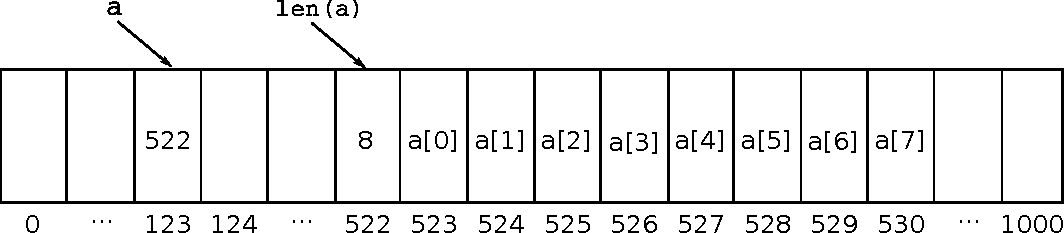
\includegraphics[scale=0.4]{figures/list_rep.pdf}}
\end{center}
\end{frame}

\begin{frame}[fragile]
\pause

Lists are mutable objects because we can change their values

\pause
\bigskip

For example, the following code reverses the order of elements in a list \lstinline{a}

\begin{lstlisting}[language=Python]
n = len(a)
for i in range(n / 2):
    temp = a[i]
    a[i] = a[n - 1 - i]
    a[n - 1 - i] = temp
\end{lstlisting}

\pause
\bigskip

One of the most basic operations on a list is to iterate over all its elements

\pause
\bigskip

For example, the following code computes the average of a list of floats

\begin{lstlisting}[language=Python]
total = 0.0
for i in range(len(a)):
    total += a[i]
average = total / len(a)
\end{lstlisting}

\pause

and the following code does the same without referring to the indices explicitly

\begin{lstlisting}[language=Python]
total = 0.0
for v in a:
    total += v
average = total / len(a)
\end{lstlisting}
\end{frame}

\begin{frame}[fragile]
\pause

Python has several built-in functions that take lists as arguments

\pause
\bigskip

For example, given a list \lstinline{a}
\begin{itemize}
\item \lstinline{len(a)} returns the number of elements in the list
\item \lstinline{sum(a)} returns the sum of the elements in the list
\item \lstinline{min(a)} returns the minimum element in the list
\item \lstinline{max(a)} returns the maximum element in the list
\item ...
\end{itemize}

\pause
\bigskip

We can write a list by passing it as an argument to \lstinline{stdio.write()} or \lstinline{stdio.writeln()}, or we can use a \lstinline{for} statement to write each element individually

\pause
\bigskip

Aliasing refers to the situation where two variables refer to the same object

\pause
\bigskip

For example, after the assignment statements
\begin{lstlisting}[language=Python]
x = [.30, .60, .10]
y = x
x[1] = .99
\end{lstlisting}
the value of \lstinline{y[1]} is also \lstinline{.99}
\end{frame}

\begin{frame}[fragile]
\pause

One way to make a copy \lstinline{y} of a given list \lstinline{x} is to iterate though \lstinline{x} to build \lstinline{y}
\begin{lstlisting}[language=Python]
y = []
for v in x:
    y += [v]
\end{lstlisting}

\pause
\bigskip

Alternatively, the expression \lstinline{a[i:j]}, called slicing,  evaluates to a new list whose elements are \lstinline{a[i], ..., a[j - 1]}; the default value for \lstinline{i} is \lstinline{0} and the default value for \lstinline{j} is \lstinline{len(a)}, so \lstinline{y = x[:]} is equivalent to the code above

\pause
\bigskip

The \lstinline{stdarray} module from the authors of the IPP text defines functions for processing lists

\begin{center}
\begin{tabular}{cc}
function & description \\ \hline
\lstinline$stdarray.create1D(n, val)$ & list of length $n$, each element initialized to $val$ \\
\lstinline$stdarray.create2D(m, n, val)$ & $m$-by-$n$ list, each element initialized to $val$ \\
$\dots$ & $\dots$
\end{tabular} 
\end{center}

\pause
\bigskip

The \lstinline{sys.argv} object that we have been using to read command-line arguments is a list of string objects
\end{frame}

\begin{frame}[fragile]
\pause

\begin{framed}
\tiny Example: Code for representing and processing playing cards.
\end{framed}

\pause

Represent suits and ranks
\begin{lstlisting}[language=Python]
SUITS = ['Clubs', 'Diamonds', 'Hearts', 'Spades']
RANKS = ['2', '3', '4', '5', '6', '7', '8', '9', '10', 
         'Jack', 'Queen', 'King', 'Ace']
\end{lstlisting}

\pause

Write a random card name
\begin{lstlisting}[language=Python]
rank = random.randrange(0, len(RANKS))
suit = random.randrange(0, len(SUITS))
stdio.writeln(RANKS[rank] + ' of ' + SUITS[suit])
\end{lstlisting}

\pause

Create a deck
\begin{lstlisting}[language=Python]
deck = []
for rank in RANKS:
    for suit in SUITS:
        card = rank + ' of ' + suit
        deck += [card]
\end{lstlisting}

\pause

Shuffle the deck
\begin{lstlisting}[language=Python]
n = len(deck)
for i in range(n):
    r = random.randrange(i, n)
    temp = deck[r]
    deck[r] = deck[i]
    deck[i] = temp
\end{lstlisting}
\end{frame}

\begin{frame}[fragile]
\pause

\begin{framed}
\tiny sample.py: Accept integers $m$ and $n$ as command-line arguments. Write to standard output a random sample of $m$ integers in the range $0 \dots n-1$ (no duplicates).
\end{framed}

\begin{lstlisting}[language=Python]
import random
import stdarray
import stdio
import sys

m = int(sys.argv[1])
n = int(sys.argv[2])
perm = stdarray.create1D(n, 0)
for i in range(n):
    perm[i] = i
for i in range(m):
    r = random.randrange(i, n)
    temp = perm[r]
    perm[r] = perm[i]
    perm[i] = temp
for i in range(m):
    stdio.write(str(perm[i]) + ' ')
stdio.writeln()
\end{lstlisting}

\pause

\begin{lstlisting}[language={}]
$ python sample.py 6 16
9 6 0 8 5 15 
$ python sample.py 10 1000
389 22 385 925 611 485 866 978 212 298 
$ python sample.py 20 20
7 18 2 16 4 10 14 0 3 13 17 8 5 1 11 6 9 12 19 15 
\end{lstlisting}
\end{frame}

\begin{frame}[fragile]
\pause

\begin{framed}
\tiny couponcollector.py: Accept integer $n$ as a command-line argument. Write to standard output the number of coupons you collect before obtaining one of each of $n$ types.
\end{framed}

\begin{lstlisting}[language=Python]
import random
import stdarray
import stdio
import sys

n = int(sys.argv[1])
count = 0
collectedCount = 0
isCollected = stdarray.create1D(n, False)
while collectedCount < n:
    value = random.randrange(0, n)
    count += 1
    if not isCollected[value]:
        collectedCount += 1
        isCollected[value] = True
stdio.writeln(count)
\end{lstlisting}

\pause

\begin{lstlisting}[language={}]
$ python couponcollector.py 1000
5821
$ python couponcollector.py 1000
8155
$ python couponcollector.py 1000000
13988284
\end{lstlisting}
\end{frame}

\begin{frame}[fragile]
\pause

\begin{framed}
\tiny primesieve.py: Accept integer $n$ as a command-line argument. Write to standard output the number of primes less than or equal to $n$.
\end{framed}

\begin{minipage}{160pt}
\begin{lstlisting}[language=Python]
import stdarray
import stdio
import sys

n = int(sys.argv[1])
isPrime = stdarray.create1D(n + 1, True)
for i in range(2, n):
    if (isPrime[i]):
        for j in range(2, n / i + 1):
            isPrime[i * j] = False
count = 0
for i in range(2, n + 1):
    if isPrime[i]:
        count += 1
stdio.writeln(count)
\end{lstlisting}

\end{minipage}%
\begin{minipage}{140pt}
\hfill \visible<2->{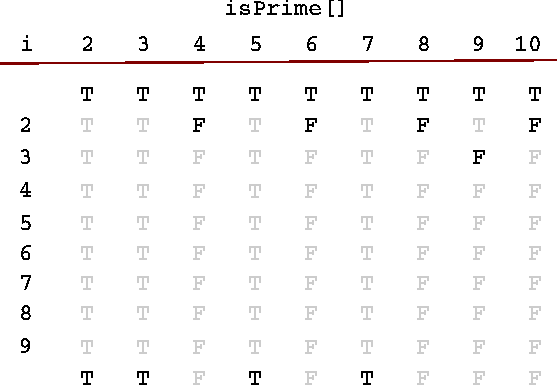
\includegraphics[scale=0.5]{figures/sieve.pdf}}
\end{minipage}

\pause

\begin{lstlisting}[language={}]
$ python primesieve.py 25
9
$ python primesieve.py 100
25
$ python primesieve.py 10000
1229
$ python primesieve.py 1000000
78498
$ python primesieve.py 100000000
5761455
\end{lstlisting}
\end{frame}

\begin{frame}[fragile]
\pause

In many applications, a convenient way to store information is to use a table of numbers organized in a rectangular table and refer to rows and columns in the table

\pause
\bigskip

The simplest way to create a two-dimensional list in Python is to place comma-separated one-dimensional lists between matching square brackets 

\pause
\bigskip

For example, this matrix of integers having two rows and three columns 
\[
\begin{bmatrix}
18 & 19 & 20 \\ 
21 & 22 & 23
\end{bmatrix}
\]
can be represented in Python using this list of lists
\begin{lstlisting}[language=Python]
a = [[18, 19, 20], [21, 22, 23]]
\end{lstlisting}

\pause
\bigskip

Python represents an $m$-by-$n$ list as a list that contains $m$ objects, each of which is a list that contains $n$ objects

\pause
\bigskip

For example, the following code creates an $m$-by-$n$ list \lstinline{a} of floats, with all elements initialized to \lstinline{0.0}
\begin{lstlisting}[language=Python]
a = []
for i in range(m):
    row = [0.0] * n
    a += [row]
\end{lstlisting}
\end{frame}

\begin{frame}[fragile]
\pause

When \lstinline{a} is a two-dimensional list, the syntax \lstinline{a[i]} refers to its \lstinline{i}th row, which is a one-dimensional list; The syntax \lstinline{a[i][j]} refers to the object at row \lstinline{i} and column \lstinline{j}

\pause
\bigskip

For example, the following code adds two $n$-by-$n$ matrices \lstinline{a} and \lstinline{b}

\begin{lstlisting}[language=Python]
c = stdarray.create2D(n, n, 0.0)
for i in range(n):
    for j in range(n):
        c[i][j] = a[i][j] + b[i][j]
\end{lstlisting}
\end{frame}

\begin{frame}[fragile]
\pause

\begin{framed}
\tiny selfavoid.py: Accept integers $n$ and $trials$ as command-line arguments. Do $trials$ random self-avoiding walks in an $n$-by-$n$ lattice. Write to standard output the percentage of dead ends encountered.
\end{framed}

\begin{minipage}{190pt}
\begin{lstlisting}[language=Python]
import random
import stdarray
import stdio
import sys

n      = int(sys.argv[1])
trials = int(sys.argv[2])
deadEnds = 0
for t in range(trials):
    a = stdarray.create2D(n, n, False)
    x = n / 2
    y = n / 2
    while (x > 0) and (x < n - 1) and 
          (y > 0) and (y < n - 1):
        a[x][y] = True
        if a[x - 1][y] and a[x + 1][y] and 
           a[x][y - 1] and a[x][y + 1]:
            deadEnds += 1
            break
        r = random.randrange(1, 5)
        if   (r == 1) and (not a[x + 1][y]):
            x += 1
        elif (r == 2) and (not a[x - 1][y]):
            x -= 1
        elif (r == 3) and (not a[x][y + 1]):
            y += 1
        elif (r == 4) and (not a[x][y - 1]):
            y -= 1
stdio.writeln(str(100 * deadEnds / trials) + 
              '% dead ends')
\end{lstlisting}
\end{minipage}%
\begin{minipage}{110pt}
\hfill \visible<2->{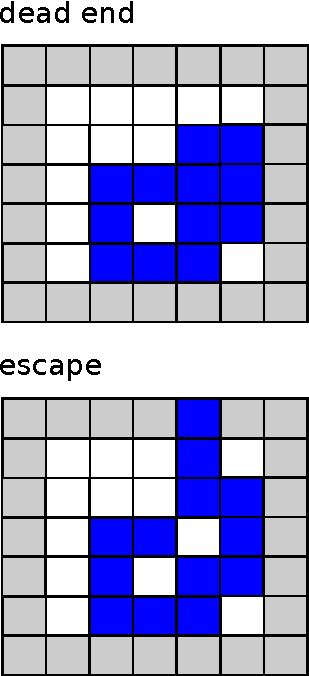
\includegraphics[scale=0.45]{figures/selfavoid.pdf}}
\end{minipage}
\end{frame}

\begin{frame}[fragile]
\pause

\begin{lstlisting}[language={}]
$ python selfavoid.py 5 100
0% dead ends
$ python selfavoid.py 20 100
31% dead ends
$ python selfavoid.py 40 100
77% dead ends
$ python selfavoid.py 80 100
98% dead ends
$ python selfavoid.py 5 1000
0% dead ends
$ python selfavoid.py 20 1000
30% dead ends
$ python selfavoid.py 40 1000
75% dead ends
$ python selfavoid.py 80 1000
98% dead ends
\end{lstlisting}
\end{frame}

\begin{frame}[fragile]
\pause

A list with rows of nonuniform length is known as a ragged list

\pause
\bigskip

For example, the following code writes the contents of a ragged list

\begin{lstlisting}[language=Python]
for i in range(len(a)):
    for j in range(len(a[i])):
        stdio.write(a[i][j])
        stdio.write(' ')
    stdio.writeln()
\end{lstlisting}

\pause
\bigskip

The same notation extends to allow us to compose code using lists that have any number of dimensions

\pause
\bigskip

For example, using lists of lists of lists, we can create a three-dimensional list \lstinline{a}, and then refer to an individual element of \lstinline{a} as \lstinline{a[i][j][k]}
\end{frame}

\section{Tuples}
\begin{frame}[fragile]
\pause

A tuple (an object of the built-in sequence type \lstinline{tuple}) consists of a number of values separated by commas
\begin{lstlisting}[language={}]
>>> t = 12345, 54321, 'hello!'
>>> t[0]
12345
>>> t
(12345, 54321, 'hello!')
\end{lstlisting}

\pause
\bigskip

Tuples may be nested
\begin{lstlisting}[language={}]
>>> u = t, (1, 2, 3, 4, 5)
>>> u
((12345, 54321, 'hello!'), (1, 2, 3, 4, 5))
\end{lstlisting}

\pause
\bigskip

Tuples are immutable, but they can contain mutable objects
\begin{lstlisting}[language={}]
>>> v = ([1, 2, 3], [3, 2, 1])
>>> v
([1, 2, 3], [3, 2, 1])
\end{lstlisting}

\pause
\bigskip

Empty and singleton sequences
\begin{lstlisting}[language={}]
>>> empty = ()
>>> singleton = 'hello', 
>>> len(empty)
0
>>> len(singleton)
1
\end{lstlisting}

\pause
\bigskip

Sequence unpacking
\begin{lstlisting}[language={}]
>>> x, y, z = t
\end{lstlisting}
\end{frame}

\section{Sets}
\begin{frame}[fragile]
\pause

A set (an object of the built-in sequence type \lstinline{set}) is an unordered collection with no duplicate elements
\begin{lstlisting}[language={}]
>>> basket = ['apple', 'orange', 'apple', 'pear', 'orange', 'banana']
>>> fruit = set(basket)
>>> fruit
set(['orange', 'pear', 'apple', 'banana'])
\end{lstlisting}

\pause
\bigskip

Fast membership testing
\begin{lstlisting}[language={}]
>>> 'orange' in fruit
True
>>> 'crabgrass' in fruit
False
\end{lstlisting}

\pause
\bigskip

Set operations
\begin{lstlisting}[language={}]
>>> a = set('abracadabra')
>>> b = set('alacazam')
>>> a                                  # unique letters in a
set(['a', 'r', 'b', 'c', 'd'])
>>> a - b                              # letters in a but not in b
set(['r', 'd', 'b'])
>>> a | b                              # letters in either a or b
set(['a', 'c', 'r', 'd', 'b', 'm', 'z', 'l'])
>>> a & b                              # letters in both a and b
set(['a', 'c'])
>>> a ^ b                              # letters in a or b but not both
set(['r', 'd', 'b', 'm', 'z', 'l'])
\end{lstlisting}
\end{frame}

\section{Dictionaries}
\begin{frame}[fragile]
\pause

A dictionary (an object of the built-in mapping type \lstinline{dict}) is an unordered set of key-value pairs, with the requirement that the keys are unique
\begin{lstlisting}[language={}]
>>> tel = {'jack': 4098, 'sape': 4139}
>>> tel['guido'] = 4127
>>> tel
{'sape': 4139, 'guido': 4127, 'jack': 4098}
>>> tel['jack']
4098
>>> tel['irv'] = 4127
>>> tel
{'guido': 4127, 'irv': 4127, 'jack': 4098, 'sape': 4139}
>>> 'guido' in tel
True
\end{lstlisting}

\pause
\bigskip

Dictionaries can be built directly from sequences of key-value pairs
\begin{lstlisting}[language={}]
>>> dict([('sape', 4139), ('guido', 4127), ('jack', 4098)])
{'sape': 4139, 'jack': 4098, 'guido': 4127}
\end{lstlisting}
\end{frame}

\section{Comprehensions}
\begin{frame}[fragile]
\pause

Comprehensions provide a concise way to create collections

\pause
\bigskip

List comprehensions
\begin{lstlisting}[language={}]
>>> squares = [x ** 2 for x in range(10)]
>>> squares
[0, 1, 4, 9, 16, 25, 36, 49, 64, 81]
>>> [(x, y) for x in [1, 2, 3] for y in [3, 1, 4] if x != y]
[(1, 3), (1, 4), (2, 3), (2, 1), (2, 4), (3, 1), (3, 4)]
\end{lstlisting}

\pause
\bigskip

Nested list comprehensions
\begin{lstlisting}[language={}]
>>> matrix = [
...     [1, 2, 3, 4],
...     [5, 6, 7, 8],
...     [9, 10, 11, 12],
... ]
>>> [[row[i] for row in matrix] for i in range(4)]
[[1, 5, 9], [2, 6, 10], [3, 7, 11], [4, 8, 12]]
\end{lstlisting}

\pause
\bigskip

Set comprehensions
\begin{lstlisting}[language={}]
>>> a = {x for x in 'abracadabra' if x not in 'abc'}
>>> a
set(['r', 'd'])
\end{lstlisting}

\pause
\bigskip

Dictionary comprehensions
\begin{lstlisting}[language={}]
>>> {x: x ** 2 for x in (2, 4, 6)}
{2: 4, 4: 16, 6: 36}
\end{lstlisting}
\end{frame}

\section{Looping Techniques}
\begin{frame}[fragile]
\pause

When looping through a sequence, the position index and corresponding value can be retrieved at the same time using the \lstinline{enumerate()} function
\begin{lstlisting}[language={}]
>>> for i, v in enumerate(['tic', 'tac', 'toe']):
...     stdio.writeln(str(i) + ' ' + v)
...
0 tic
1 tac
2 toe
\end{lstlisting}

\pause
\bigskip

To loop over two or more sequences at the same time, the entries can be paired with the \lstinline{zip()} function
\begin{lstlisting}[language={}]
>>> questions = ['name', 'quest', 'favorite color']
>>> answers = ['lancelot', 'the holy grail', 'blue']
>>> for q, a in zip(questions, answers):
...     stdio.writeln('What is your ' + q + '? It is ' + a)
...
What is your name? It is lancelot.
What is your quest? It is the holy grail.
What is your favorite color? It is blue.
\end{lstlisting}
\end{frame}

\begin{frame}[fragile]
\pause

To loop over a sequence in reverse, first specify the sequence in a forward direction and then call the \lstinline{reversed()} function
\begin{lstlisting}[language={}]
>>> for i in reversed(range(1, 10, 2)):
...     stdio.writeln(i)
...
9
7
5
3
1
\end{lstlisting}

\pause
\bigskip

To loop over a sequence in sorted order, use the \lstinline{sorted()} function which returns a new sorted list while leaving the source unaltered
\begin{lstlisting}[language={}]
>>> basket = ['apple', 'orange', 'apple', 'pear', 'orange', 'banana']
>>> for f in sorted(set(basket)):
...     stdio.writeln(f)
...
apple
banana
orange
pear
\end{lstlisting}
\end{frame}
\end{document}
